% AISM 2026 submission.
% VENUE FACTS: every preamble fact below was fetched from the call for papers, not recalled.
% AISM 2026 is co-located with ASE 2026, Munich, Germany, 12-16 October 2026.
% Review is SINGLE-BLIND, so this paper is NOT anonymised. Template is the ACM Primary Article
% Template in sigconf format, as required by the ASE 2026 Research Track submission page.
% Limit: 8 pages INCLUDING references.
\documentclass[sigconf]{acmart}

% Included figure PDFs otherwise leave their include path in the shipped PDF bytes as
% /PTEX.FileName; suppress all PTEX provenance comments.
\pdfsuppressptexinfo=-1

\usepackage{booktabs}
\usepackage{tikz}
\usetikzlibrary{positioning,arrows.meta,calc}
% Long identifiers set in \texttt do not hyphenate, and in a narrow two-column measure they push
% a line into the margin. Two such boxes (2.19pt and 5.30pt) predate this revision; naming the
% exact model checkpoints so a reader can pin them added a third at 83pt. \emergencystretch gives
% TeX extra stretch on a final pass, and ONLY for a paragraph that would otherwise be overfull,
% so paragraphs that already set cleanly are untouched. Verified by rebuilding and counting: the
% count goes 2 to 0, and the reference list does not move.
\setlength{\emergencystretch}{1.5em}
\usepackage{balance}

% GENERATED by code/make_macros.py from data/results.json. Do not edit by hand.
% Regenerate after every analysis run; the build is not valid without it.
\newcommand{\NAmendments}{10}
\newcommand{\NHumanEval}{164}
\newcommand{\NSigEligible}{147}
\newcommand{\NProblems}{136}
\newcommand{\NDropped}{11}
\newcommand{\NFuzz}{1000}
\newcommand{\MutantFloor}{90}
\newcommand{\KParity}{10}
\newcommand{\NModels}{5}
\newcommand{\NCells}{1583}
\newcommand{\NUsable}{510}
\newcommand{\NDivergent}{165}
\newcommand{\DivRate}{32.4}
\newcommand{\UsableQwen}{114}
\newcommand{\DivQwen}{33.3}
\newcommand{\UsableDsCoder}{105}
\newcommand{\DivDsCoder}{35.2}
\newcommand{\UsableMistral}{58}
\newcommand{\DivMistral}{63.8}
\newcommand{\UsableLlama}{97}
\newcommand{\DivLlama}{40.2}
\newcommand{\UsableGemini}{136}
\newcommand{\DivGemini}{10.3}
\newcommand{\EscapeRate}{40.8}
\newcommand{\EscapeLo}{32.8}
\newcommand{\EscapeHi}{49.2}
\newcommand{\NEscaped}{425}
\newcommand{\NPassed}{1041}
\newcommand{\EscapeQwen}{49.5}
\newcommand{\EscapeDsCoder}{50.3}
\newcommand{\EscapeMistral}{50.8}
\newcommand{\EscapeLlama}{42.2}
\newcommand{\EscapeGemini}{14.9}
\newcommand{\EscapeOrdinary}{7.7}
\newcommand{\EscapeOrdinaryLo}{4.2}
\newcommand{\EscapeOrdinaryHi}{11.9}
\newcommand{\NEscapedOrdinary}{80}
\newcommand{\OrdinaryShare}{46.3}
\newcommand{\EscapeOracleOnly}{13.0}
\newcommand{\NEscapedOracleOnly}{135}
\newcommand{\NRepairedTranslations}{27}
\newcommand{\NRepairedLlama}{21}
\newcommand{\EscapeExclRepaired}{40.8}
\newcommand{\EscapeTransQwen}{47.2}
\newcommand{\EscapeTransDsCoder}{46.1}
\newcommand{\EscapeTransMistral}{56.0}
\newcommand{\EscapeTransLlama}{36.3}
\newcommand{\EscapeTransGemini}{32.2}
\newcommand{\SelfMiss}{54.3}
\newcommand{\SelfMissLo}{45.1}
\newcommand{\SelfMissHi}{63.3}
\newcommand{\SelfMissN}{164}
\newcommand{\CrossMiss}{48.4}
\newcommand{\CrossMissLo}{41.2}
\newcommand{\CrossMissHi}{55.4}
\newcommand{\CrossMissN}{690}
\newcommand{\MissDiff}{5.9}
\newcommand{\MissDiffLo}{-0.1}
\newcommand{\MissDiffHi}{12.2}
\newcommand{\PermGroups}{153}
\newcommand{\PermSelfMiss}{52.3}
\newcommand{\PermCrossMiss}{48.6}
\newcommand{\PermDiff}{3.7}
\newcommand{\PermP}{0.603}
\newcommand{\DiagMiss}{54.3}
\newcommand{\OffDiagMiss}{48.4}
\newcommand{\PseudoDiagMiss}{49.6}
\newcommand{\DiagPerms}{120}
\newcommand{\DiagP}{0.18}
\newcommand{\DiagDiff}{4.7}
\newcommand{\DiagNullLo}{40.1}
\newcommand{\DiagNullHi}{58.9}
\newcommand{\VMissQwen}{56.9}
\newcommand{\VMissDsCoder}{63.9}
\newcommand{\VMissMistral}{75.6}
\newcommand{\VMissLlama}{59.0}
\newcommand{\VMissGemini}{11.0}
\newcommand{\THardQwen}{51.5}
\newcommand{\THardDsCoder}{48.4}
\newcommand{\THardMistral}{28.7}
\newcommand{\THardLlama}{35.7}
\newcommand{\THardGemini}{84.2}
\newcommand{\BestValidatorMiss}{11.0}
\newcommand{\HardestTranslatorMiss}{84.2}
\newcommand{\WorstCellMiss}{89.6}
\newcommand{\WorstCellN}{48}
\newcommand{\WVValidators}{5}
\newcommand{\WVWorseOnOwn}{2}
\newcommand{\WVMeanDiff}{-6.3}
\newcommand{\PairTranslations}{309}
\newcommand{\PairAllFive}{10}
\newcommand{\PairMedian}{3}
\newcommand{\TargetTimeouts}{259}
\newcommand{\CovEscapes}{130}
\newcommand{\CovSamePath}{86.2}
\newcommand{\NTraceFailed}{5}
\newcommand{\MissCrossLang}{29.6}
\newcommand{\MissLogic}{17.4}
\newcommand{\MissIntWidth}{71.9}
\newcommand{\CrossExIntMiss}{21.6}
\newcommand{\NAttempted}{680}
\newcommand{\NCompiled}{539}
\newcommand{\NCompileFail}{141}
\newcommand{\NNoComparable}{29}
\newcommand{\RegCells}{854}
\newcommand{\RegOR}{0.90}
\newcommand{\RegORLo}{0.68}
\newcommand{\RegORHi}{1.14}
\newcommand{\NBootRegression}{2,000}
\newcommand{\RegP}{0.38}
\newcommand{\GeeOR}{0.89}
\newcommand{\GeeP}{0.29}
\newcommand{\MatchTrans}{153}
\newcommand{\MatchSelfMiss}{52.3}
\newcommand{\MatchCrossMiss}{48.6}
\newcommand{\MatchSelfN}{153}
\newcommand{\MatchCrossN}{364}
\newcommand{\MatchP}{0.42}
\newcommand{\DropSelf}{34.7}
\newcommand{\DropCross}{42.9}
\newcommand{\DropWorseSelfN}{3}
\newcommand{\DropValidatorsChecked}{5}
\newcommand{\DiagPUnion}{0.38}
\newcommand{\EscapeTwoLo}{20.7}
\newcommand{\EscapeTwoHi}{61.2}
\newcommand{\JackLo}{34.8}
\newcommand{\JackHi}{52.3}
\newcommand{\CfourDropped}{11}
\newcommand{\CfourNondet}{0}
\newcommand{\ConeTags}{11}
\newcommand{\ConeMismatch}{0}
\newcommand{\WVWorseOnOwnUnion}{2}
\newcommand{\WVMeanDiffUnion}{-9.4}
\newcommand{\SelfEscape}{37.6}
\newcommand{\CrossEscape}{41.8}
\newcommand{\EscapeKThree}{50.2}
\newcommand{\SelfMissKThree}{69.1}
\newcommand{\CrossMissKThree}{58.6}
\newcommand{\EscapeKFive}{46.7}
\newcommand{\SelfMissKFive}{62.2}
\newcommand{\CrossMissKFive}{52.6}
\newcommand{\EscapeKTen}{40.8}
\newcommand{\SelfMissKTen}{45.3}
\newcommand{\CrossMissKTen}{43.6}
\newcommand{\TargetedMiss}{53.8}
\newcommand{\PlainMiss}{52.5}
\newcommand{\TargetedGain}{1.3}
\newcommand{\TargetedPairs}{158}
\newcommand{\TargetedOnlyWin}{1}
\newcommand{\TargetedOnlyLoss}{3}
\newcommand{\TargetedP}{0.625}
\newcommand{\RandomEscape}{52.0}
\newcommand{\RandomCells}{500}
\newcommand{\RandomMiss}{65.4}
\newcommand{\RandomMissN}{312}
\newcommand{\LlmMissAll}{49.6}
\newcommand{\LlmMissN}{847}
\newcommand{\RandomMissUnion}{65.4}
\newcommand{\LlmMissUnion}{44.0}
\newcommand{\RandomMissOracle}{33.3}
\newcommand{\LlmMissOracle}{25.7}
\newcommand{\ComboMissLlm}{49.5}
\newcommand{\ComboMissRandom}{59.5}
\newcommand{\ComboMissBoth}{40.9}
\newcommand{\ComboGain}{8.6}
\newcommand{\ComboOnlyLlm}{159}
\newcommand{\ComboOnlyRandom}{74}
\newcommand{\ComboCells}{854}
\newcommand{\OnlySuiteFound}{151}
\newcommand{\DivTransUnion}{315}
\newcommand{\DivTransOracle}{164}
\newcommand{\OnlySuiteShare}{47.9}
\newcommand{\NSuites}{2695}
\newcommand{\NUnparseable}{85}
\newcommand{\NDegenerate}{1026}
\newcommand{\PctUnparseable}{3.2}
\newcommand{\EscapeWithDegenerate}{48.5}
\newcommand{\NCallFailed}{1}
\newcommand{\DegenQwen}{272}
\newcommand{\UnparseQwen}{6}
\newcommand{\DegenDsCoder}{97}
\newcommand{\UnparseDsCoder}{9}
\newcommand{\DegenMistral}{390}
\newcommand{\UnparseMistral}{70}
\newcommand{\DegenLlama}{232}
\newcommand{\UnparseLlama}{0}
\newcommand{\DegenGemini}{35}
\newcommand{\UnparseGemini}{0}
\newcommand{\MedianSrc}{-0.5}
\newcommand{\MedianTgt}{0.0}
\newcommand{\MedianDiverge}{1}
\newcommand{\MedianComparable}{999}
\newcommand{\MaxTokensPerCall}{1,024}
\newcommand{\CallRetries}{5}
\newcommand{\BoundaryFraction}{0.30}
\newcommand{\NScalarIntBoundaries}{15}
\newcommand{\NElemExtraBoundaries}{7}
\newcommand{\NFloatBoundaries}{14}
\newcommand{\NStrBoundaries}{17}
\newcommand{\MaxStrBoundaryLen}{200}
\newcommand{\ListShapeProb}{0.4}
\newcommand{\GcdInA}{-139}
\newcommand{\GcdInB}{6}
\newcommand{\GcdSrc}{1}
\newcommand{\GcdTgt}{-1}
\newcommand{\GcdDiverge}{221}
\newcommand{\GcdComparable}{1,000}
\newcommand{\GcdPassedValidators}{2}
\newcommand{\GcdUsableSuites}{4}
\newcommand{\GcdCaughtValidators}{2}
\newcommand{\IntReturning}{60,819}
\newcommand{\OutOfRange}{2,098}
\newcommand{\OutOfRangeProblems}{25}
\newcommand{\CtwoMutants}{151}
\newcommand{\CtwoKill}{94.0}
\newcommand{\CtwoBenchKill}{87.4}
\newcommand{\CtwoGapPP}{6.6}
\newcommand{\CthreeN}{20}
\newcommand{\CthreeCaught}{18}
\newcommand{\CthreeEquivalent}{2}
\newcommand{\CthreeGenuineMiss}{0}
\newcommand{\CthreeExtraInputs}{7,998}
\newcommand{\BenchDetect}{50.3}
\newcommand{\BenchDetected}{83}
\newcommand{\BenchDivergent}{165}
\newcommand{\BenchInputsMean}{9}
\newcommand{\CfiveChecked}{510}
\newcommand{\CfiveViolations}{0}
\newcommand{\NClassified}{165}
\newcommand{\CrossLangShare}{69.1}
\newcommand{\LogicShare}{30.9}
\newcommand{\NCrossLang}{114}
\newcommand{\CrossLangQwen}{71.1}
\newcommand{\CrossLangDsCoder}{70.3}
\newcommand{\CrossLangMistral}{56.8}
\newcommand{\CrossLangLlama}{74.4}
\newcommand{\CrossLangGemini}{78.6}
\newcommand{\TaxNameOne}{other logic}
\newcommand{\TaxPctOne}{30.9}
\newcommand{\TaxNameTwo}{string handling}
\newcommand{\TaxPctTwo}{26.7}
\newcommand{\TaxNameThree}{integer width}
\newcommand{\TaxPctThree}{10.3}
\newcommand{\TaxTopThree}{67.9}
          % generated from ../data/results.json by code/make_macros.py; never edit
% GENERATED by code/make_macros.py. Do not edit by hand.
\newcommand{\SummaryBody}{%
Qwen2.5 7B & 114 & 38 & 33.3 & 49.5 \\
DS-Coder 6.7B & 105 & 37 & 35.2 & 50.3 \\
Mistral 7B & 58 & 37 & 63.8 & 50.8 \\
Llama 3 8B & 97 & 39 & 40.2 & 42.2 \\
Gemini 3.6 F & 136 & 14 & 10.3 & 14.9 \\
}
\newcommand{\MatrixHead}{Qwen2.5 & DS-Coder & Mistral & Llama & Gemini}
\newcommand{\MatrixBody}{%
Qwen2.5 & \textbf{54} & 67 & 48 & 35 & 79 \\
DS-Coder & 73 & \textbf{66} & 40 & 50 & 90 \\
Mistral & 73 & 73 & \textbf{25} & 78 & 80 \\
Llama & 60 & 66 & 31 & \textbf{45} & 81 \\
Gemini & 15 & 14 & 2 & 11 & \textbf{44} \\
}
\newcommand{\TaxonomyBody}{%
other logic & 51 & 30.9 \\
string handling & 44 & 26.7 \\
integer width & 17 & 10.3 \\
negative division rounding & 15 & 9.1 \\
collection ordering & 11 & 6.7 \\
target exception:ArrayIndexOutOfBoundsException & 9 & 5.5 \\
target exception:StringIndexOutOfBoundsException & 7 & 4.2 \\
\midrule
6 further categories & 11 & 6.7 \\
\textbf{total} & \textbf{165} & \textbf{100.0} \\
}
           % likewise: table bodies are generated, not typed

% ACM rights block, inserted VERBATIM from ACM's Publication Release Confirmation
% (received 2026-09-01). Do not tidy the spacing inside
% \acmConference/\acmBooktitle: it is ACM's own string. If the upload checker objects and
% offers its own block, that one supersedes this wholesale (it also carries
% \acmSubmissionID and \received lines).
\copyrightyear{2026}
\acmYear{2026}
\setcopyright{cc}
\setcctype{by}
\acmConference[AISM '26 ]{Proceedings of the 2nd International Workshop on AI for Software Modernization }{October 12--16, 2026}{Munich, Germany}
\acmBooktitle{Proceedings of the 2nd International Workshop on AI for Software Modernization (AISM '26 ), October 12--16, 2026, Munich, Germany}
\acmDOI{10.1145/3843775.3844550}
\acmISBN{979-8-4007-2987-4/2026/10}

\begin{document}

\title{Passing Parity Is Not Preserving Behaviour: Oracle Escape in
       Function-Level LLM Code Migration}

% CAMERA-READY author block, aligned with the ACM eRights form (2026-08-31). The form's
% "Email" field is the contact address printed here; its separate "Institutional Email" field
% carries the author's institutional address, which is what ACM uses for institutional
% attribution and ACM Open APC coverage. City is deliberately not declared, matching the
% checker-clean configuration of the author's other ASE 2026 workshop papers.
\author{Simarjot Khanna}
\email{simarkhanna76@gmail.com}
\affiliation{%
  \institution{Independent Researcher}
  \country{Canada}
}

\begin{abstract}
Parity testing validates software modernization: the legacy system supplies every expected
output, so the oracle is sound. One decision is delegated, increasingly to a language model and
often the very model that translated the code: which inputs to try. How much divergence such
suites let through is unmeasured, and whether a model validating its own translation misses
more is unknown; we pre-registered that self-validation hypothesis. We measure both in
Python-to-Java function migration with five models, each acting as both translator and
validator, with expected values always from executing the legacy source and divergence
established by differential execution on a large type-directed input set together with the
generated suites. Of the parity suites that passed, \EscapeRate\% were on divergent
translations, and \EscapeOrdinary\% on translations that diverge on an input a reviewer would
call unremarkable. We could not detect a self-validation penalty. Validator strength and translator
subtlety dominate instead: misses are worst when a weak validator checks a strong translator's
code, the configuration a cost-conscious pipeline prefers. A passing parity suite is evidence
about where testing has looked, not a verdict of behavioural equivalence, and should be
reported with its escape rate attached.
\end{abstract}

\keywords{software modernization, code migration, semantic preservation, test oracles,
          large language models, parity testing}

\maketitle

\section{Introduction}

Automated modernization has stopped being a translation problem and become a trust problem.
Production pipelines translate COBOL to Java at enterprise
scale~\cite{chakravarthy2026enterprise} and upgrade Java repositories
agentically~\cite{liu2025migrationbench}. Deployment turns on whether the output can be shown
to behave like the system it replaces, not on whether it compiles.

Legacy estates rarely come with tests, so validation manufactures its own. The construction the
field has converged on is \emph{parity testing}: pick inputs, run the legacy system for the
expected outputs, run the migrated system, and compare. Symbolic execution
has been used to pick those inputs for COBOL~\cite{kumar2024validation,hans2025testing}, and an
agentic loop has been proposed that searches for them under deterministic parity
checks~\cite{ferenczi2026locksmith}.

Nothing here depends on a model predicting what the program \emph{should} do; the legacy system
answers that. Exactly one thing is delegated, increasingly to a language model: the choice of
\emph{which inputs to try}. Throughout, the \emph{translator} is the model that produced the
translation and the \emph{validator} is the model that chooses the parity inputs checking it;
the two are often the same model.

We ask what that delegation costs: when an LLM-generated parity suite passes, how often is the
migration divergent anyway, and does the answer depend on who wrote the suite? That
measurement, against a ground truth the suites did not define, is the contribution.

Our design isolates the question. Every model acts as both translator and validator, so the
matrix of pairings has a self-validation diagonal and a cross-validation off-diagonal, and
expected values always come from executing the source, so the only free variable is where the
validator looks. Pairing is partial: a divergent translation is scored by however many
validators produced a usable suite for it, a median of \PairMedian{} of \NModels{}, and the
analysis is built around that. Section~3 gives the full design and the oracle's measured
detection power.

\paragraph{What this study is and is not.}
We study Python-to-Java migration of short, self-contained functions. That is not a legacy
estate, and we claim no numerical carry-over to a COBOL modernization. We chose this setting
because it is the smallest one admitting a differential oracle at all: at repository scale
there is no ground truth to score a parity suite against, which is why the question has not
been answered. What transfers is the \emph{principle} the oracle rests on:
expected values are deferred to the legacy system while input selection is delegated. The
shape of the result transfers too: a language pair has a gap class of its own, and generic
testing is worst precisely there. The engineering does not transfer: a stateful estate needs
mocked resources, replayed I/O and trace-level
comparison~\cite{kumar2024validation,ferenczi2026locksmith}. Its language pair will also have
gap categories of its own, and a pipeline should go looking for them.

\noindentparagraph{Contributions.}
\vspace{-1ex}
{\setlength{\itemsep}{0pt}\setlength{\parsep}{0pt}
\begin{itemize}
\item An escape-rate measurement for migration validation: across \NCells{}
      validator-translator-problem cells, \EscapeRate\% of the LLM-generated parity suites
      that passed were on divergent translations (95\% CI \EscapeLo--\EscapeHi), and
      \EscapeOrdinary\% on translations that diverge on an unremarkable input; under the
      independent oracle alone, \EscapeOracleOnly\%.
\item Evidence on correlated blindness: no detectable self-validation penalty, from miss
      rates tested pairwise within translation.
\item A grounded taxonomy of what escapes, built from observed divergences rather than
      synthetic mutants.
\item Three mitigations evaluated against the same ground truth, and a public replication
      package\footnote{\url{https://github.com/s1mar/parity-escape}} that runs on one
      workstation.
\end{itemize}}

\section{Background and Related Work}

\paragraph{LLM-assisted migration.}
Production modernization pipelines now combine static analysis with language models. IBM's
enterprise COBOL-to-Java pipeline pairs program analysis with LLMs and is evaluated by an
automated LLM-as-judge on twenty GenAPP programs and ten customer
apps~\cite{chakravarthy2026enterprise}. \textsc{MigrationBench} frames repository-level
Java~8 upgrades as an agentic task over 5,102 repositories~\cite{liu2025migrationbench}. At the
first edition of this workshop, migration and modernization tasks ranged from COBOL functionality
extraction~\cite{rajbhoj2025cobol} to automated dependency upgrades~\cite{tawosi2025dependency}.

\paragraph{Deciding that a migration preserved behaviour.}
Kumar et
al.~\cite{kumar2024validation} generate COBOL unit tests by symbolic execution, mock external
resource calls, and emit matching JUnit tests; the same group reports a testing framework built
around this idea for IBM watsonx Code Assistant for Z~\cite{hans2025testing}. A recent preprint
describes the ``Locksmith Loop''~\cite{ferenczi2026locksmith}, which makes input selection
\emph{agentic}: an LLM
loop searches for inputs that penetrate program branches, and accepted translations are those
that match the source under deterministic parity checks. Across all of these the expected value
is never in doubt; what differs is which inputs are tried. Our results
project onto these systems directly: any input-selection mechanism, whether a symbolic
executor, an agentic search loop or a prompted model, can be scored by the share of divergent
translations its accepted suites let through, measured against divergences it did not itself
establish. That is the evaluation this paper applies to LLM selectors, and nothing in its
construction is specific to LLMs.

\paragraph{How much do such suites actually detect?}
Test-adequacy studies exist for code \emph{generation} benchmarks. EvalPlus expands HumanEval's
tests by 80$\times$ and finds that pass@k drops by up to 19.3--28.9\% once the extra inputs are
applied~\cite{liu2023evalplus}, and Liu et al.~\cite{liu2025adequacy} study the test adequacy of
execution-based generation benchmarks directly. Translation corpora are weaker still: AVATAR
pairs 9,515 Java and Python programs but supplies unit tests for only
250~\cite{ahmad2021avatar}. Rabbi et al.~\cite{rabbi2026beyond} examine 6,164 translations and
show that many reported \emph{failures} are artifacts of misconfigured evaluation. That result is
the mirror image of ours: they show reported failures overstate the defect count, we ask whether
reported passes overstate correctness.

\paragraph{Blind spots in self-assessment.}
Language models assess their own output poorly. In a secure-code repair study, Gong et
al.\ report that GPT-3.5 and GPT-4 ``both perform poorly when repairing self-produced code,
indicating self-repair `blind spots'\,''~\cite{gong2024secure}. Zhao et
al.~\cite{zhao2026misguidance} show that exposure to
buggy code makes a model assert the erroneous behaviour and suppresses bug-finding tests. Both
concern what the model \emph{claims}, the expected value; migration validation removes exactly
that freedom. Whether a blind spot
survives when only \emph{input selection} is left to the model is, to our knowledge,
untested, and it is the
question this paper answers. Meta-validation of judges in low-data modernization
settings has been raised at this workshop before~\cite{fandina2025vintage}; we take the
complementary execution-based route.

\section{Study Design}

The design is fixed in a pre-registration written before any model was called; it is included in
the replication package together with its \NAmendments{} recorded amendments, each with the reason
and the direction of its effect.

\begin{figure}[t]
\centering
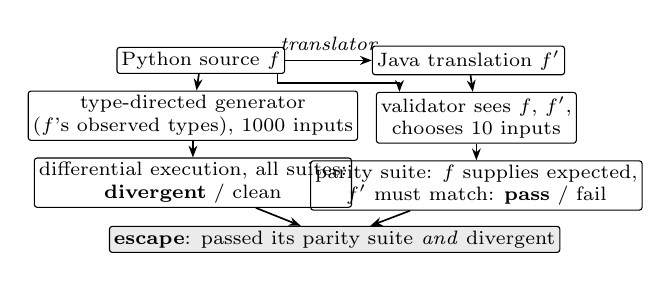
\begin{tikzpicture}[
  font=\scriptsize,
  box/.style={draw, rounded corners=1pt, align=center, inner sep=1.6pt},
  arr/.style={-{Stealth[length=1.5mm]}, semithick}
]
\node[box] (src) {Python source $f$};
\node[box, right=11mm of src] (tgt) {Java translation $f'$};
\draw[arr] (src) -- node[above, font=\scriptsize\itshape] {translator} (tgt);
\node[box, below=2.1mm of src, xshift=-1mm] (gen) {type-directed generator\\ ($f$'s observed types), \NFuzz{} inputs};
\node[box, below=2.1mm of tgt, xshift=1mm] (val) {validator sees $f$, $f'$,\\ chooses \KParity{} inputs};
\draw[arr] (src) -- (gen);
\draw[arr] (tgt) -- (val);
\draw[arr] (src.south east) ++(-1mm,0) |- ($(val.north west)+(3mm,1.1mm)$) -- ($(val.north west)+(3mm,0)$);
\node[box, below=2.1mm of gen] (dif) {differential execution, all suites:\\ \textbf{divergent} / clean};
\node[box, below=2.1mm of val] (par) {parity suite: $f$ supplies expected,\\ $f'$ must match: \textbf{pass} / fail};
\draw[arr] (val) -- (par);
\draw[arr] (gen) -- (dif);
\node[box, fill=black!8, below=2.1mm of $(par.south)!0.5!(dif.south)$]
  (esc) {\textbf{escape}: passed its parity suite \emph{and} divergent};
\draw[arr] (par) -- (esc);
\draw[arr] (dif) -- (esc);
\end{tikzpicture}
\caption{The pipeline, run per (validator, translator, problem) cell; an escape is a
divergent translation whose parity suite passed.}
\label{fig:pipeline}
\end{figure}

\paragraph{Study design at a glance.}
\NProblems{} Python functions; \NModels{} models; one translation per (model, problem) and one
parity suite per (validator, translation), giving \NCells{} scorable validator-translator-problem cells
(Figure~\ref{fig:pipeline}). Two input sets play different roles. The \KParity{} model-chosen
inputs per suite, with expected outputs from executing the Python source, are the object under
test. Differential execution on \NFuzz{} type-directed inputs per
problem, unioned with the generated suites themselves, supplies the ground truth the suites are
scored against. Both compare the translation to the source; they differ in role, not in kind. A
translation \emph{escapes} when its parity suite passes while the translation is divergent
under the ground truth; a validator \emph{misses} a divergent translation when its suite passes
on it.

\subsection{Set-up}

We treat a Python function as the legacy source and Java as the modernization target. Java is
the destination language of the enterprise pipelines this work is about; Python stands in for
the legacy source, which in those pipelines is COBOL, as a dynamically typed language with a
public corpus carrying executable tests. The corpus is the HumanEvalPack Python
split~\cite{muennighoff2024octopack}, itself derived from HumanEval~\cite{chen2021codex}
(\NHumanEval{} problems). Most HumanEval signatures carry no return annotation, so rather than
parse types we \emph{observe} them: the benchmark's own test block is executed with the entry
point replaced by a recording proxy, which yields the concrete argument and return types and the
benchmark's own inputs. \NSigEligible{} problems have types our marshalling layer supports;
\NDropped{} more are dropped because their source is nondeterministic under repeated execution or
because too few generated inputs are in domain, leaving \NProblems{}.

Translations are produced by \NModels{} models spanning distinct families: four run locally
under Ollama (\texttt{qwen2.5:\allowbreak 7b-\allowbreak instruct},
\texttt{deepseek-\allowbreak coder:\allowbreak 6.7b-\allowbreak instruct},
\texttt{mistral:\allowbreak 7b-\allowbreak instruct-\allowbreak v0.2-\allowbreak q4\_0},
\texttt{llama3:\allowbreak latest}) and one is a hosted frontier model
(\texttt{gemini-\allowbreak 3.6-\allowbreak flash-\allowbreak high}, queried 7 August 2026).
Every model acts as \emph{both}
translator and validator, giving a square matrix whose diagonal is self-validation. Decoding is
fixed at temperature~0.2 and top-p~0.95, with seed~0 on the local route (the hosted route
exposes no seed control). Every call allows \MaxTokensPerCall{} output tokens, one sample per
cell, and up to \CallRetries{} retries with exponential backoff that fire only on a transport
failure or an empty response, never on content.

The translator is handed the source and an \emph{exact} Java method signature derived
mechanically from the observed types, and must implement it. Fixing the signature removes
signature ambiguity as a confound and lets one reflective JSON harness serve every problem.
The one exception: a translation failing to compile solely for missing imports gets a fixed
import preamble, nothing else (\NRepairedTranslations{} of \NAttempted{} attempted,
\NRepairedLlama{} of them Llama~3's). Compile counts are post-repair, and excluding every
repaired translation leaves the escape rate at \EscapeExclRepaired\%. Python \texttt{int} maps to Java \texttt{long}: no
fixed-width type is faithful to an arbitrary-precision integer, and \texttt{long} is the
conservative choice because it makes overflow \emph{harder} to produce than \texttt{int} would.

\subsection{The thing under test: a parity suite}

Each validator receives the source and a candidate translation and returns \KParity{} test
\emph{inputs} as JSON argument tuples. It is never asked for an expected value. The prompt
shows both programs, states that expected values will come from executing the legacy source,
and asks for the inputs ``most likely to expose a behavioural difference between the two
programs, if one exists''; the verbatim template is in the replication package. Expected values
come from executing the Python source on those inputs. A translation \emph{passes} if its output matches
the source on every in-domain input. Inputs on which the source raises are out of domain; a suite
leaving fewer than three in-domain inputs is recorded as degenerate and reported separately
rather than counted as a silent pass.

\subsection{Ground truth: the strong oracle}

Divergence is decided by differential execution on \NFuzz{} type-directed inputs per problem,
which include the benchmark's own inputs as a prefix, so the strong oracle is a strict superset
of the benchmark-provided one. The generator's rule is fixed and mechanical, with one seed for
the whole study. After the benchmark prefix, each generated input is flagged \emph{boundary}
with probability \BoundaryFraction. A boundary input draws every argument from a fixed per-type
catalogue: \NScalarIntBoundaries{} small signed integers when the integer is a scalar argument,
joined by \NElemExtraBoundaries{} values near
$2^{31}$, $2^{63}$ and $10^{18}$ when it sits inside a list, where magnitude feeds the
function's arithmetic rather than an allocation size. The float catalogue holds
\NFloatBoundaries{} values including signed zero, $10^{-9}$ and $10^{18}$; the string catalogue
\NStrBoundaries{}, including the empty string, whitespace, non-ASCII text and a
\MaxStrBoundaryLen-character string. Boundary lists have
length 0, 1, 2 or 100, and with probability \ListShapeProb{} are made all-equal, sorted, or
reverse-sorted. A non-boundary input draws each argument from tiered magnitude ranges, small
values weighted most; the catalogues and tiers are constants in the replication
package. A translation is \textsc{divergent} if any in-domain input yields a
different output. Integers compare exactly, floats to a relative tolerance of $10^{-6}$, and a
target exception where the source returned a value counts as divergence.

Resource exhaustion does not. Timeouts, out-of-memory conditions and oversize results are
excluded on both sides, because a Java heap limit says nothing about whether behaviour was
preserved. Excluding them can only remove candidate divergences, so every rate we report is a
lower bound.

One class of artifact needs care, because a fixed signature can force a difference the model
could not have avoided. Types are observed on the benchmark's own inputs, so a fuzz input can
take the source somewhere those observations never went: \texttt{largest\_divisor} returns an
\texttt{int} on every benchmark input and \texttt{None} on a negative one, which no Java method
returning a primitive can reproduce. We therefore treat any input on which the source returns a
value that is not \emph{representable in the declared Java type} as out of domain.
Representability, not merely type: Python integers are unbounded and the declared type is
\texttt{long}, so a source that legitimately computes a value beyond $2^{63}-1$ would force the
translation to differ whatever the model wrote, because we fixed the signature. That case
accounts for \OutOfRange{} of \IntReturning{} integer-returning source outputs across
\OutOfRangeProblems{} problems, and all of them are excluded. The same rule covers the
neighbouring cases: a source returning a float where \texttt{int} was inferred is out of domain
rather than a divergence, no Python value is ever mapped to a Java \texttt{char}, and a problem
whose element type cannot be resolved (an always-empty collection) never enters the corpus at all.

What the rule deliberately does \emph{not} exclude is a source whose result \emph{is}
representable while the target's arithmetic diverges on the way there. Those are avoidable by a
careful translation, so they are real defects. None of the width-related divergences we report
has an out-of-range source value or an \emph{ordinary} witness, so the conservative
\EscapeOrdinary\% rate of Section~\ref{sec:rqone} does not depend on the integer mapping.

\subsection{Controls}

An instrument that detects nothing would report a clean zero escape rate and read as a null
result, so the oracle's power is measured rather than asserted.
\textbf{C1} round-trips every supported type through the marshalling harness and requires exact
equality, isolating marshalling bugs from translation bugs.
\textbf{C2} seeds single-token mutants of the legacy source (comparison-operator swaps,
arithmetic swaps, constant increments) and reports what share the strong oracle kills, against
what share the benchmark's own inputs kill on the same mutants.
\textbf{C3} injects a known divergence into translations the oracle called clean and requires
it to flip.
\textbf{C4} executes every source twice and excludes any problem whose outputs differ, because
parity against a nondeterministic source is meaningless.
\textbf{C5} exploits a strict impossibility: the random baseline draws its inputs \emph{from} the
strong oracle's own input list, so a divergence it reports must also appear in the oracle's
verdict for the same translation. Any violation would indict the fuzzer, the marshalling, the
domain rules or the comparison predicate, exercised through two independently written code paths.

\subsection{Metrics and statistics}
\label{sec:metrics}

We report two rates. \textsc{Escape rate} is the share of parity-passing translations that are
divergent: the practitioner-facing number, though its denominator moves with translator quality.
\textsc{Miss rate} is the share of \emph{divergent} translations whose parity suite failed to
catch them; it conditions on the translation, so a divergent translation is compared across the
validators that produced a usable suite for it, at most one of which wrote it. That takes
translator quality out of the contrast, which the escape rate cannot do.

Formally, index the scorable cells by $(v,t,p)$: validator $v$'s suite for translator $t$'s
translation of problem $p$. Let $S(v,t,p)\in\{0,1\}$ indicate that the suite passed, and let
$D(t,p)\in\{0,1\}$ indicate that the translation is divergent, meaning the strong oracle or any
generated suite exhibited an in-domain input on which target and source outputs differ. Then
\begin{align*}
\text{escape rate} &= \frac{\bigl|\{(v,t,p): S{=}1,\ D{=}1\}\bigr|}
                          {\bigl|\{(v,t,p): S{=}1\}\bigr|}
  = \Pr\bigl[D{=}1 \mid S{=}1\bigr],\\[2pt]
\text{miss rate} &= \frac{\bigl|\{(v,t,p): S{=}1,\ D{=}1\}\bigr|}
                        {\bigl|\{(v,t,p): D{=}1\}\bigr|}
  = \Pr\bigl[S{=}1 \mid D{=}1\bigr].
\end{align*}
For the self-validation comparison of Section~\ref{sec:rqtwo}, the divergence indicator is
\emph{leave-one-out}: $D_{-v}(t,p)=1$ only when the oracle or a suite written by some validator
other than $v$ witnessed a divergence, so a selector's own catches never help define the set it
is scored against.

Confidence intervals come from a cluster bootstrap over problems (10,000 resamples;
\NBootRegression{} for the regression of Section~\ref{sec:rqtwo}), since
translations of one problem are not independent. Three hypothesis tests appear in this paper; the fixed-effects regression and the GEE
reported beside RQ2 are estimation views of the same contrast, not further tests. The pre-registered one is a paired permutation test (10,000 permutations)
reshuffling which validator carries the ``self'' label within a translation; we report it but do
not rely on it, because validators are not exchangeable and it is therefore confounded. The test
we rely on for RQ2 is an exact permutation over the \DiagPerms{} column permutations of the
matrix, which holds every row and column marginal fixed. RQ4 uses an exact McNemar test on paired
cells. Our pre-registration declared only the first of these; the second is a recorded
amendment, written before any RQ2 number had been computed.

\section{Results}

\subsection{Does the instrument work?}
\label{sec:instrument}

All five controls pass; two produce results in their own right.

Marshalling round-trips exactly for all \ConeTags{} supported type tags, with \ConeMismatch{}
mismatches (C1). Nondeterminism is a declared exclusion reason that never fired: all
\CfourDropped{} dropped problems fell to the in-domain floor and \CfourNondet{} to
nondeterminism (C4). The strong oracle kills \CtwoKill\% of \CtwoMutants{} seeded
single-token mutants of the legacy source (C2), above the \MutantFloor\% floor fixed in advance.
It flags \CthreeCaught{} of \CthreeN{} injected divergences (C3); both survivors are relational
boundary flips that produced no divergence against \CthreeExtraInputs{} further
differently-seeded inputs, so they are very likely equivalent mutants and C3 is better read as
\CthreeCaught{} of \CthreeCaught{} non-equivalent injections. C5 exploits a strict
impossibility, that the random baseline draws its inputs from the oracle's own list: over
\CfiveChecked{} scorable cells there are \CfiveViolations{} violations.

Two of these numbers matter beyond instrument validation.

\textbf{Source-language mutation adequacy does not predict translation detection.} The
benchmark's own test inputs, a mean of \BenchInputsMean{} per problem, kill \CtwoBenchKill\% of
the same source mutants: the extra \NFuzz{} fuzz inputs buy \CtwoGapPP{} more points. Yet those
same inputs detect only \BenchDetect\% of the \BenchDivergent{} translations that actually
diverge (\BenchDetected{} of them). The comparison is deliberately between two different things,
and that is the point: a suite scored against mutants of the \emph{source} can look strong while
missing nearly half the defects introduced by \emph{translation}, because a single-token source
mutant sits
at a site the suite already exercises and a cross-language divergence sits where the two
languages disagree. Two limits on that claim. We did not mutate the Java translations, so this is
about the adequacy measure computed on the legacy program, not about mutation testing in general.
And our operators are single-token; a richer operator set, or a system-level suite of the kind an
enterprise estate carries, could close some of the gap. What the numbers rule out is treating a
high source-side score as evidence that a migration has been validated.

\textbf{Our own oracle is incomplete, and we report it rather than repair it.} Counting
translations that any method showed to be divergent, \DivTransUnion{} in total,
\OnlySuiteFound{} were witnessed only by a generated parity suite and never by the
\NFuzz{}-input oracle, which independently identified \DivTransOracle{}. (That is one fewer than
the \NDivergent{} in Table~\ref{tab:summary}: one divergent translation had no validator produce
a scorable suite for it, so it cannot enter any cell-level count.) The reason is visible in the inputs: a model probes a bracket matcher with
\texttt{"~(~(~a~)~)~(~b~)~"}, a structured string the type-directed generator never emits. We did
not strengthen the generator after seeing this, because tuning an instrument towards a larger
headline number is not a defensible move. Instead, ground truth for RQ1 is the union $D$ of the
oracle and every suite, and RQ2 uses the leave-one-out rule $D_{-v}$ of
Section~\ref{sec:metrics}, the only rule clean in both directions;
Section~\ref{sec:rqtwo} reports the two one-sided alternatives beside it. \NFuzz{} random
type-directed inputs miss divergences that ten chosen inputs find, so for this task input
\emph{selection} matters more than input \emph{volume}.

\subsection{RQ1: how much passes that should not}
\label{sec:rqone}

Across \NCells{} scorable validator-translator-problem cells, \NEscaped{} of the \NPassed{}
passing cells sit on a divergent translation: an escape rate of \EscapeRate\%
(95\% CI \EscapeLo--\EscapeHi). The unit is the cell, so a divergent translation contributes
one escape per validator whose suite passed it. Under the oracle's witnesses alone the rate is
\EscapeOracleOnly\% (\NEscapedOracleOnly{} cells); the union counts a divergence on \emph{any}
in-domain input as real. That is residual risk conditional on a pass: of the sign-offs this validation produced, this
share was divergent. It is not the cost \emph{caused} by delegating to a model: at the same budget the
non-LLM baseline of Section~\ref{sec:rqfour} misses more, not fewer, of the same divergences.

That interval clusters on problems, treating the five models as fixed. Two checks bound the
model dimension. Dropping each model
in turn, as both translator and validator, the escape rate ranges from \JackLo\% to \JackHi\%,
highest when Gemini is removed: no single model produces the effect. Resampling models as well
as problems widens the interval to \EscapeTwoLo--\EscapeTwoHi\%. That dimension is coarse with
five models; a reader who wants to generalise beyond this ensemble should use the wider
interval.

The aggregate hides who wrote the suite. Escape rate by
validator runs from \EscapeGemini\% for Gemini to \EscapeMistral\% for Mistral, with the three
other open models between \EscapeLlama\% and \EscapeDsCoder\%. For a team generating its parity
inputs with a small local model, roughly one in two of the migrations it signs off is divergent.

Three things are excluded from the denominator rather than counted as passes, because a
validator should not look safe by failing to produce a usable suite. \NDegenerate{} of
\NSuites{} suites left fewer than three in-domain inputs and are recorded as degenerate;
\NUnparseable{} (\PctUnparseable\%) could not be parsed into argument tuples at all;
\NCallFailed{} more was lost to a failed model call. The extremes are far apart: Gemini produced \DegenGemini{} degenerate suites and \UnparseGemini{} unparseable
ones, Mistral \DegenMistral{} and \UnparseMistral{}. The exclusion is conservative: counting degenerate parseable suites as passes unless they
caught something raises the escape rate to \EscapeWithDegenerate\%.

More inputs help, but slowly. Taking prefixes of the same generated suites, the escape rate is
\EscapeKThree\% at $K{=}3$, \EscapeKFive\% at $K{=}5$ and \EscapeKTen\% at $K{=}10$. Tripling the
budget removes about ten points of escape; one cannot test one's way out at that rate.

One escape shows the shape of the problem. For \texttt{median},
Gemini validated its own translation with ten inputs that included \texttt{[MAX]},
\texttt{[MAX,\,MAX]} and \texttt{[MIN,\,MIN]}: it was plainly thinking about 64-bit limits. It
never tried \texttt{[MAX,\,MIN]}, and on that input the source returns \texttt{\MedianSrc} while
the translation returns \texttt{\MedianTgt}.

The mechanism is not the obvious one, and nothing overflows: $2^{63}-1$ has no exact
\texttt{double} representation, so widening each \texttt{long} to \texttt{double} rounds it up
to $2^{63}$, the two extremes cancel to exactly zero, and the division returns zero. Python's unbounded integers and true \texttt{/} do neither. The
case looks like overflow and like truncating integer division, and is neither.

The suite passed. The divergence appears on \MedianDiverge{} of \MedianComparable{} comparable
inputs, so a slightly larger sample would not have found it by luck.

Finally, the conservative reading. Restricting to divergences that have at least one
\emph{ordinary} witness input, meaning no integer above $10^3$ in magnitude anywhere in the
input, no string longer than 25 characters or containing non-ASCII, and no list longer than 20
elements, the escape rate falls to \EscapeOrdinary\% of passing cells
(95\% CI \EscapeOrdinaryLo--\EscapeOrdinaryHi); \NEscapedOrdinary{} of the \NEscaped{} escapes have
such a witness, every one of them oracle-witnessed. So roughly one in thirteen parity-passing
sign-offs is wrong on an input a reviewer would call unremarkable, and roughly two in five are
wrong on some input.

\begin{table}[t]
\caption{Per model: translations the harness could execute, how many diverge from the source
under the strong oracle, and the escape rate, under the union ground truth of
Section~\ref{sec:instrument}, when that model acts as \emph{validator}.}
\label{tab:summary}
\small
\begin{tabular}{lrrrr}
\toprule
Model & usable & diverg. & diverg.\% & escape\% \\
\midrule
\SummaryBody
\bottomrule
\end{tabular}
\end{table}

\subsection{RQ2: does it matter who wrote the suite}
\label{sec:rqtwo}

\begin{figure}[t]
\centering
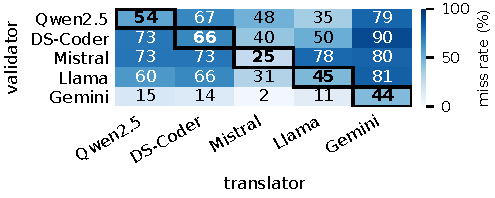
\includegraphics[width=\linewidth]{fig_matrix}
\caption{Miss rate (\%) on \emph{divergent} translations, each cell annotated with its value
to the nearest whole point. Rows: the validator that chose the inputs; columns: the
translator that wrote the code; boxed diagonal: self-validation. The visible structure is a
pale bottom row (its own boxed self-cell aside) and a dark right column, not a dark diagonal.}
\label{fig:matrix}
\end{figure}

\textbf{We could not detect it, and we had predicted we would.} On divergent translations the raw
miss rate is \SelfMiss\% under self-validation ($n{=}\SelfMissN$) against \CrossMiss\% under
cross-validation ($n{=}\CrossMissN$), a gap of \MissDiff{} points (95\% CI $\MissDiffLo$ to
$\MissDiffHi$, an interval that includes zero). That raw gap is exactly the confounded comparison: the
diagonal is populated by a different mix of validators and translators than the off-diagonal, so
it cannot be read as an effect.

Two estimation views that do control it agree. A logistic regression over all \RegCells{} divergent cells,
with fixed effects for validator identity and for translator identity and an indicator for
self-validation, puts the odds ratio on missing under self-validation at \RegOR{}
(95\% CI \RegORLo--\RegORHi{}, cluster bootstrap over problems, $p{=}\RegP$); a logistic GEE with
an exchangeable working correlation clustered on problem gives \GeeOR{} ($p{=}\GeeP$). Both point
slightly \emph{below} one, meaning if anything a small self-validation advantage, and neither is
distinguishable from no effect. These views handle the very unequal cell sizes natively,
which the permutation below cannot.

The amended primary test tells the same story: the observed diagonal sits \DiagDiff{}
points above the mean pseudo-diagonal, well inside the null range \DiagNullLo--\DiagNullHi\%,
$p{=}\DiagP$ over all \DiagPerms{} permutations. Its caveat is the converse: column permutation does not weight the pseudo-diagonal quite as
the true diagonal is weighted across cells of four to sixty-two observations, hence the
estimation views beside it. The pre-registered paired test also agrees ($p{=}\PermP$).

We report all of this as a failure to detect rather than a demonstration of absence: a penalty
smaller than this design resolves could exist.

Ground truth here is the leave-one-out rule $D_{-v}$ of Section~\ref{sec:metrics}. That
matters, because the two obvious alternatives are biased in opposite directions, and we report
both. Scoring on
oracle-confirmed divergences only favours the random baseline, whose inputs are drawn from the
oracle's own list; scoring on the full union favours the model validators, whose own catches
would help define the set. Leave-one-out has a residual cost of its own, in exactly the direction
that matters here: it discards a catch that \emph{only} the scored validator made, which is what
a genuine self-recognition advantage would look like. That bias runs \emph{against} the null we
report, so it cannot have manufactured it, and we report the union beside it regardless. Under
leave-one-out, \WVWorseOnOwn{} of \WVValidators{} validators are worse on their own translations,
mean difference $\WVMeanDiff$ points; under the union, \WVWorseOnOwnUnion{} of \WVValidators{},
mean $\WVMeanDiffUnion$ points. The exact matrix test is null under both
($p{=}\DiagP$ leave-one-out, $p{=}\DiagPUnion{}$ union). The conclusion is the same under all three.

One more asymmetry could produce a spurious null: differential dropout between own and foreign
code would leave the surviving diagonal and off-diagonal describing different populations. Pooled across all cells, dropout does differ: \DropSelf\% of self cells are lost to degenerate
or unparseable suites against \DropCross\% of cross cells. That gap is not a validator tendency:
\DropWorseSelfN{} of \DropValidatorsChecked{} validators drop out \emph{more} on their own
translations, the opposite direction.

Restricting to the
\MatchTrans{} divergent translations that have both a usable self suite and at least one usable
cross suite (the same translations the pre-registered paired test operates on), every
translation contributes to both conditions and differential dropout cannot apply. On that matched subsample the miss rate is \MatchSelfMiss\% self ($n{=}\MatchSelfN$)
against \MatchCrossMiss\% cross ($n{=}\MatchCrossN$), and the exact matrix test gives
$p{=}\MatchP$. The null survives a design in which attrition is impossible.

One apparent exception: Gemini misses far more of the divergences in its own translations than
in other models', which looks like self-blindness. It is not. Gemini's translations are hardest
for \emph{everyone} (other validators miss \THardGemini\%, against \THardMistral--\THardQwen\%
for the other four) and Gemini itself misses fewer of them than any other validator does. That
is a column effect, which the permutation over columns is built to absorb.

\paragraph{What the matrix does show.}
Two large associations, neither of which is self-validation (Figure~\ref{fig:matrix}). We describe
them rather than claim to have isolated them: this is an observational matrix, and translator
identity bundles capability, defect mix and problem coverage together.

Along the rows, miss rate varies by \emph{validator}: measured only on other models'
translations, Gemini misses \VMissGemini\% while the four open models miss \VMissQwen\% to
\VMissMistral\%. Along the columns, it varies by \emph{whose translation is being checked}, from
\THardMistral\% for Mistral up to \THardGemini\% for Gemini, and that ordering tracks translator
quality: the divergences a better model leaves behind are the harder ones to catch.

Those two run in opposite directions, and the cell where both are unfavourable is the one a
cost-conscious pipeline is most likely to build: a strong model to translate, a cheap model to
check it; it is the worst cell we observe. DeepSeek-Coder validating Gemini's translations misses
\WorstCellMiss\% of them ($n{=}\WorstCellN$). A 7B validator does not see roughly nine in ten of
a frontier translator's divergences, and the reason is not that it is checking its own work.

\subsection{RQ3: what diverges}

The \NModels{} arms attempted \NAttempted{} translations, \NModels{} per problem.
\NCompileFail{} never compiled and \NNoComparable{} more compiled but produced no comparable
output, leaving \NUsable{} executable. Compile failures are a visible defect that a pipeline
catches for free, so they are excluded from every rate below rather than counted as escapes; the
loss is uneven across arms and Table~\ref{tab:summary} gives it per model. Of the executable
translations \NDivergent{}
(\DivRate\%) diverge from the source under the strong oracle. The taxonomy classifies exactly
these, because its rules read the triples of the oracle's differential runs; the larger union
of Section~\ref{sec:instrument} adds suite-only witnesses without such runs.
Divergence tracks model capability in the expected
direction: \DivGemini\% for Gemini, \DivQwen\% for Qwen2.5, \DivDsCoder\% for DeepSeek-Coder,
\DivLlama\% for Llama~3, \DivMistral\% for Mistral (Table~\ref{tab:summary}).

Classifying each divergence by rule from its (input, source output, target output) triple gives
Table~\ref{tab:taxonomy}. The assignment is mechanical. An ordered list of predicates over that
triple is evaluated most specific first, and the first match assigns the category; a
translation's category is the most frequent category over its divergent inputs. No model is involved, so the labels
are deterministic, and the classifier ships with an audit mode that prints randomly sampled
labelled divergences with their evidence so the labelling can be checked by hand.

The useful cut is not the individual categories but the split above
them. \CrossLangShare\% of divergences are \emph{cross-language}: they arise where Python and Java
disagree about what an operation means, so a direct or idiomatic Java implementation gets them
wrong unless it explicitly emulates the Python semantics; a target-side exception where the
source returned a value is counted here too. They are avoidable, which is why we
count them as defects; they are simply not avoided by writing the obvious code. The remainder are
ordinary logic errors, where the translation computes something else entirely.

A worked case shows what a characteristic cross-language divergence looks like, and how
ordinary its witness can be, where the \texttt{median} escape of Section~\ref{sec:rqone} was
subtle. Asked for
\texttt{greatest\_common\_divisor}, DeepSeek-Coder translated Euclid's algorithm line for line:
the loop body becomes \texttt{a1 = temp \% a1}, which is the obvious translation, and it is
wrong. Python's remainder takes the sign of the divisor; Java's takes the sign of the dividend.
On input $(\GcdInA, \GcdInB)$ the source returns $\GcdSrc$ and the translation returns
$\GcdTgt$, and the two differ on \GcdDiverge{} of \GcdComparable{} comparable inputs, broadly
those with a negative argument. Of the \GcdUsableSuites{} usable parity suites for this
translation, \GcdCaughtValidators{} caught it and \GcdPassedValidators{} passed it, one of the
passing two being DeepSeek-Coder's own: \KParity{} plausible inputs are easy to choose without
a negative first argument.

That split moves with model quality, and it moves the wrong way for anyone hoping better models
will solve this: cross-language divergences are \CrossLangMistral\% of Mistral's failures and
\CrossLangGemini\% of Gemini's. The ordering across the five is not strictly monotone, but the
endpoints are far apart and the direction is clear. As translation improves, ordinary mistakes
disappear and what remains concentrates in the semantic gap between the languages: fixed-width
integers where Python has none, floored versus truncated division of negatives, case and index
conventions on strings, and ordering of equal elements. Those are also the divergences the parity
suites are worst at finding: on oracle-confirmed divergent cells the miss rate is
\MissCrossLang\% for cross-language categories against \MissLogic\% for ordinary logic errors,
and \MissIntWidth\% for integer width alone; without integer width the remaining cross-language
cells are missed \CrossExIntMiss\%. The class that grows as translators improve is the
class validation is least able to catch.

\begin{table}[t]
\caption{Divergent translations by modal category, assigned by rule from the (input, source
output, target output) triples of their divergent runs. \CrossLangShare\% fall in
cross-language classes.}
\label{tab:taxonomy}
\small
\begin{tabular}{lrr}
\toprule
category & n & \% \\
\midrule
\TaxonomyBody
\bottomrule
\end{tabular}
\end{table}

\subsection{RQ4: what helps}
\label{sec:rqfour}

We evaluated three mitigations against the same ground truth. Two do nothing.

\textbf{Swapping to a merely \emph{different} validator bought nothing measurable}, because we
could not detect a penalty attached to identity-matching for it to remove ($p{=}\DiagP$,
Section~\ref{sec:rqtwo}). A failure to reject is not proof of absence, and a penalty below the
resolution of a five-model test could exist.

That must not be read as ``the validator does not matter'', which our data contradicts loudly:
measured on other models' translations, validator miss rate runs from \VMissGemini\% to
\VMissMistral\%. Choosing a \emph{different} model is not the intervention. Choosing a
\emph{better} one is, and it is the largest effect in this study.

\textbf{Telling the validator where to look does not help either.} We reran self-validation with
a prompt naming the cross-language classes explicitly: fixed-width overflow, floored versus
truncated division of negatives, string indexing and case, and ordering of equal elements. Over \TargetedPairs{} paired cells the miss rate moved from \PlainMiss\% to
\TargetedMiss\%, \TargetedGain{} points in the \emph{wrong} direction; across these pairs the targeted prompt
newly caught \TargetedOnlyWin{} and newly missed \TargetedOnlyLoss{} (McNemar
$p{=}\TargetedP$). For this prompt, on these cells, naming the gap classes did not turn into
inputs that land in one.

\textbf{Adding cheap generated inputs does help.} On \ComboCells{} cells, a model-chosen suite
misses \ComboMissLlm\% and \KParity{} type-directed random inputs miss \ComboMissRandom\%, but
the union of the two misses \ComboMissBoth\%, a reduction of \ComboGain{} points. The two are
complementary rather than redundant: \ComboOnlyLlm{} divergences were caught only by the model
and \ComboOnlyRandom{} only by the generator.

One asymmetry qualifies every selector comparison here: except in the matched-budget union
above, the model's \KParity{} inputs meet the generator's \NFuzz{} at their deployed budgets,
not at equal ones, and whether a much larger model-chosen budget would close the generator's
remaining margin is not answered by this design. At deployed budgets, what helped is a
different \emph{kind} of input, not a better-instructed model.

\section{Discussion}

\paragraph{Two mechanisms, and why the null is about only one.}
A self-validation penalty could arise from \emph{capability}, since a weak model writes worse
translations \emph{and} worse suites, or from \emph{correlation}, where a model's particular
misunderstanding of Java shapes both the defect it writes and the inputs it thinks worth trying.
The within-validator and matrix tests separate them by holding validator capability fixed, and
it is the correlation mechanism that they fail to find.
No self-recognition is involved either way: each validator is prompted afresh, with no memory
of the translation's origin.

\paragraph{Source-side mutation score is the wrong yardstick here.}
The benchmark's tests kill \CtwoBenchKill\% of source mutants and detect \BenchDetect\% of real
divergences; Section~\ref{sec:instrument} explains why the two measure different things. A
mutation score against the legacy program looks healthy right up to the point where it matters.

\paragraph{What we would tell a team doing this today.}
Two levers moved: validator strength (miss rates span \VMissGemini--\VMissMistral\% across
validators), and \KParity{} generated inputs beside the model's own, which removed \ComboGain{}
points of miss rate for no model call yet do not substitute for a stronger validator's far
lower residual. Run both selectors: a model probes structured, meaning-carrying inputs a
generator will not construct, and a generator probes magnitudes, empties and boundaries nobody
writes by hand, so neither subsumes the other. A better prompt moved nothing we could measure. Be most careful exactly where
intuition says to relax: a strong translator's surviving defects are the subtle ones, and a
cheap validator will not see them. That is about catching a divergence once it exists, not how
often one exists: residual risk after a pass still runs from \EscapeTransGemini\% on Gemini's
translations to \EscapeTransMistral\% on Mistral's, so the strongest translator remains the
safest source, consistent with its lowest divergence rate in Table~\ref{tab:summary}. Treat a
passing suite as evidence about where you have looked, and do not let a source-side mutation
score replace it.

\section{Threats to Validity}

\paragraph{The corpus is not a legacy estate.}
HumanEval functions are short, self-contained and pure; COBOL programs are none of these, so
the \emph{principle} transfers, not the engineering or the rates. Code size and complexity are
likely to cut both ways. On larger units a model validator must reason about more paths and
more state, while a type-directed generator needs only the signature; but the structured inputs
and program states larger code requires are exactly what blind generation is worst at
constructing. Which effect dominates cannot be answered in this design.

\paragraph{Are the divergences real defects, or unreasonable inputs?}
A translation may differ only on inputs the original author never contemplated. We take the
modernization stance that behavioural equivalence with the legacy system is the requirement,
undocumented inputs included, because legacy edge-case behaviour is routinely depended on
downstream. The \emph{ordinary}-witness rate in Section~\ref{sec:rqone} is the conservative
reading for readers who disagree.

\paragraph{Our oracle could be wrong in either direction.}
False divergences would inflate every rate: C1 round-trips every type exactly and resource
exhaustion is excluded on both sides. False equivalences would deflate them, which C2 and C3
measure rather than assume. The oracle is finite, so a translation we call clean may diverge on
an input we never tried, again making the rates lower bounds.

\paragraph{Non-termination is not counted.}
A two-second per-call limit cannot distinguish a target that loops forever from one that is
merely slower than the source, so timeouts are excluded rather than counted as divergence.
This is conservative in an uncomfortable direction: a migrated program that hangs where the
original returned is arguably the most severe failure of all, and we exclude it. All \TargetTimeouts{} target executions that timed out
where the source returned fall in translations the oracle already calls divergent, so counting
them as divergences changes no rate here.

\paragraph{Models and sampling.}
One sample per cell at temperature 0.2, four small open models and one hosted frontier model.
Different or larger models may show different rates; one sample per cell cannot separate
typical behaviour from a lucky draw. We report the frontier arm separately.
Ollama served each tag at its library default quantisation, which may not match the
reference checkpoints; the served weight digests are recorded in the replication package.

\paragraph{One shot, not an agentic search.}
Our validators are asked once for \KParity{} inputs. Deployed systems search: symbolic execution
drives COBOL test generation~\cite{kumar2024validation}, and the Locksmith
Loop~\cite{ferenczi2026locksmith} iterates until inputs penetrate branches. Coverage-driven search
would fix an escape that is merely an unexplored path. It does not obviously fix one that sits on
a path already taken, and \CovSamePath\% of the \CovEscapes{} oracle-witnessed escapes we
traced (\NTraceFailed{} of the \NEscapedOracleOnly{} resisted tracing) are of the second
kind: the divergent input executes only source lines the passing suite had already executed. What
those suites lack is not reach but the boundary value inside a line they already ran.

\paragraph{The prompt differs between conditions, unavoidably.}
A validator sees its own code on the diagonal and a stranger's off it, and those differ in length
and style. The matched subsample removes differential \emph{dropout} and the matrix test removes
row and column composition, but neither removes the possibility that a weak model reasons less
well about unfamiliar code.

\paragraph{Fixed signatures.}
Handing the translator the target signature makes our setting easier than practical migration,
and removes a confound that would otherwise dominate: without it, an incompatible signature
and a semantic divergence are indistinguishable at the harness boundary.

\section{Conclusion}

Migration validation asks a language model to decide where to look, then trusts the legacy
system to say what it should have seen. The trusted half is sound; the risk sits in the
delegated half, and not where we expected: we could detect no penalty for a model checking its
own translation rather than a stranger's. The risk is input selection treated as a detail when
it is the whole of the evidence, and getting cheaper exactly as the translations it must check
get subtler. What helped was a stronger validator, and a handful of inputs from a generator
that does not share the model's sense of a plausible input. A passing parity suite is real but
weak evidence, and belongs in a report with its escape rate attached, not as a verdict.

\section*{Data Availability}

The replication package is publicly available at
\url{https://github.com/s1mar/parity-escape}. It contains the frozen pre-registration with its
amendments, the verbatim prompts, all translations and parity suites, the oracle and control
outputs, and the scripts reproducing every number here. The corpus is
public~\cite{muennighoff2024octopack,chen2021codex} and the experiment runs on one workstation
with locally hosted models.

\section*{Use of Generative AI}

Language models are the object of study here: all translations and parity suites were
machine-generated, as described in Section~3. AI assistance was also used in implementing the
experimental harness and in preparing the manuscript. The design, the analysis and the claims
are the author's.

\balance
\bibliographystyle{ACM-Reference-Format}
\bibliography{refs}

\end{document}
